\phantomsection
\chapter[Finding Motifs in Transcription Factor Networks]{Finding Motifs in Transcription Factor Networks\chapsubhead{Noah Lee and Phillip Compeau}}
\label{chapter:motifs}
\renewcommand{\chaptertitle}{Finding Motifs in Transcription Factor Networks}
\addcontentsline{cc}{chapter}{Chapter \thechapter} % Adds chapter number to table of contents


\FloatBarrier

\section{Networks Rule (Biology)}
\label{sec:introduction}
\phantomsection

In \autoref{chapter:turing}, we worked with a particle-based model that simulated the interactions of skin cells to produce complex Turing patterns. In this chapter, we will zoom into a much lower biological scale and model protein interactions, which occur on a molecular level. The scale of these interactions is tiny: a protein is typically on the order of about 10nm in diameter. (For comparison, the diameter of a single human hair is about 100,000 nm, and a light microscope's highest resolution is about 2,000 nm.) We will see that the cell has evolved a form of molecular communication based on protein interactions that is rapid, robust, and elegant.

To model protein interactions, we will use a  \textdef{network}{network}{FILL IN}, which is a collection of \textdef{nodes}{nodes}{FILL IN} along with \textdef{edges}{edges}{FILL IN} that connect pairs of nodes. Whether we are studying the interactions of proteins, the complex chains of chemical reactions underlying cellular metabolism, the tangled webs of neurons in the human nervous system, or an evolutionary tree of life, networks are critical to our understanding of biological processes.

Our interest lies in the frequently recurring structures hidden within biological networks called \textdef{network motifs}{network motifs}{FILL IN}. Similarly to our work \autoref{chapter:turing}, we will use modeling to answer \textit{why} these motifs have evolved to help the cell respond to its environment.

We will soon define our specific network of study, but before we get ahead of ourselves, we will introduce some of the molecular biology fundamentals we will need to complete our analysis. You may already know this biological background, in which case you should feel free to skim the next section.\\

\FloatBarrier
\phantomsection

\section{Transcription and DNA-Protein Binding}
\label{sec:transcription_and_dna-protein_binding}
\phantomsection

\subsection{The central dogma of molecular biology}

DNA is a double-stranded molecule consisting of the four nucleobases adenine, cytosine, guanine, and thymine. A gene is a region of an organism's DNA that is \textdef{transcribed}{transcribed}{FILL IN} into a single-stranded RNA molecule in which thymine is converted to uracil and the other bases remain the same.

The RNA transcript is then \textdef{translated}{translated}{FILL IN} into an amino acid sequence. Because there are four different bases but twenty amino acids available, RNA is translated in \textdef{codons}{codons}{FILL IN}, or triplets of nucleobases. \autoref{fig:genetic_code} shows the way in which codons are translated into amino acids, which is called the \textdef{genetic code}{genetic code}{FILL IN}.

\begin{figure}[h]
\centering
\mySfFamily
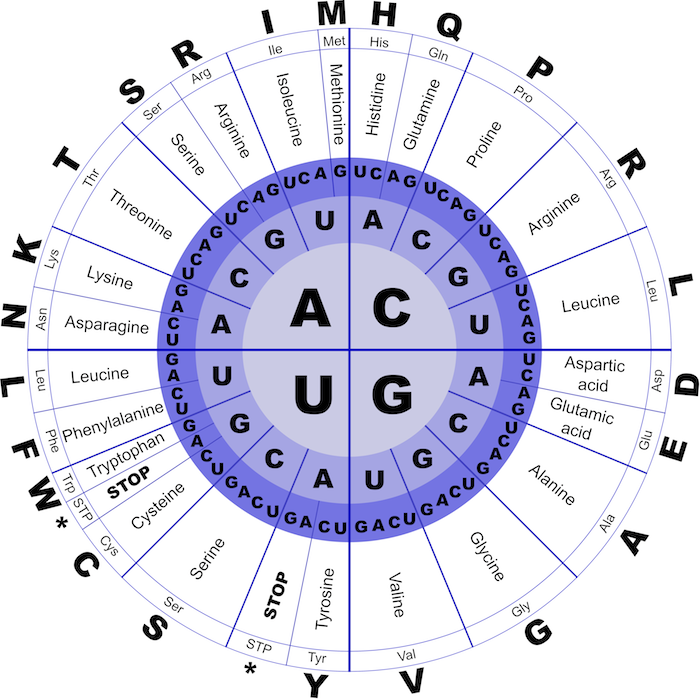
\includegraphics[width = 0.6\textwidth]{../images/genetic_code.png}
\caption{The genetic code, which dictates the conversion of RNA codons into amino acids. Codons are read from the inside of the figure outward. Image courtesy: J Alves, Open Clip Art.}
\label{fig:genetic_code}
\end{figure}

DNA can be thought of as a blueprint for storing information that flows from DNA to RNA to protein. This flow of information is called the \textdef{central dogma of molecular biology}{central dogma of molecular biology}{FILL IN}, illustrated in \autoref{fig:Central_Dogma_of_Molecular_Biochemistry_with_Enzymes}.

\begin{note}[%
Like any dogma, there are times in which the central dogma of molecular biology is violated. If you are interested in an example, consider Chapter 4 of Bioinformatics Algorithms, https://www.bioinformaticsalgorithms.org/bioinformatics-chapter-4.
]\end{note}

\begin{figure}[h]
\centering
\mySfFamily
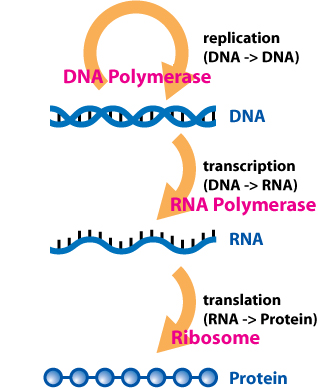
\includegraphics[width = 0.6\textwidth]{../images/Central_Dogma_of_Molecular_Biochemistry_with_Enzymes.jpg}
\caption{The central dogma of molecular biology states that molecular information flows from DNA in the nucleus, into the RNA that is transcribed from DNA, and then into proteins that are translated from RNA. Image courtesy: Dhorpool, Wikimedia commons user.}
\label{fig:Central_Dogma_of_Molecular_Biochemistry_with_Enzymes}
\end{figure}

\FloatBarrier
\phantomsection
\subsection{Transcription factors control gene regulation}

All of your cells have essentially the same DNA, and yet your liver cells, heart cells, and brain cells are able to serve different functions. This is because the rates at which these genes are \textdef{regulated}{regulated}{FILL IN}, or converted into RNA and then protein, vary between genes in different tissues.

Gene regulation typically occurs at either the DNA or protein level. At the DNA level, regulation is modulated by \textdef{transcription factors}{transcription factors}{FILL IN}, master regulator proteins that bind upstream of genes and serve to either \textdef{activate}{activate}{FILL IN} or \textdef{repress}{repress}{FILL IN} a gene's rate of transcription, turning that rate up or down, respectively.

Because of the central dogma, transcription factors are involved in a sort of feedback loop. DNA is transcribed into RNA, which is translated into the protein sequence of a transcription factor, which then binds to the upstream region of some other gene and changes its rate of transcription.

Transcription factors are vital for the cell's response to its environment because extracellular stimuli can serve to activate a transcription factor via a system of signaling molecules that convey a signal through relay molecules to the transcription factor (\autoref{fig:genetic_code}). Only when the transcription factor is activated will it regulate its target protein(s).

\begin{figure}[h]
\centering
\mySfFamily
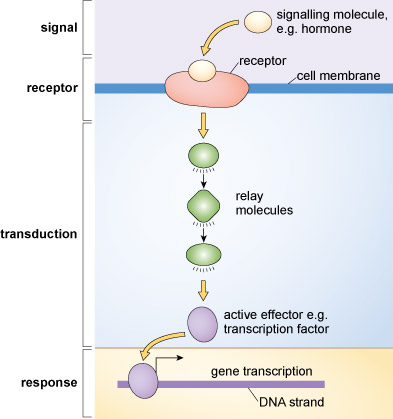
\includegraphics[width = 0.6\textwidth]{../images/signal_pathway.jpg}
\caption{A cell receiving a signal which triggers a response in which this signal is ``transduced'' into the cell, resulting in transcription of a gene. We will discuss signal transduction in greater detail in a future section.}
\label{fig:genetic_code}
\end{figure}

In \autoref{chapter:chemotaxis}, we will discuss the details of how the cell detects an extracellular signal and conveys it as a response within the cell. For now, we will focus on the relationship between transcription factors and the genes they regulate.

\FloatBarrier
\phantomsection
\subsection{Determining if a given transcription factor regulates the expression of a given gene}

Over the years, a number of both computational and experimental approaches have been developed to identify the collection of genes that a given transcription factor regulates.

A transcription factor has a weak binding affinity to DNA in general, but it has a very strong binding affinity for a single specific short sequence of nucleotides called a \textdef{motif}{motif}{FILL IN}. Think of a transcription factor as latching onto DNA and then ``sliding'' up and down the DNA molecule until it finds its target motif, where it clamps down. If this motif occurs immediately before a gene, then the transcription factor will regulate this gene.

A natural question, then, is to find the set of genes to which a transcription factor binds. A widespread experimental practice for determining where a protein bonds in an organism's genome (i.e., its total collection of DNA) is called \textdef{ChIP-seq}{ChIP-seq}{FILL IN}, which is short for \textdef{chromatin immunoprecipitation sequencing}{chromatin immunoprecipitation sequencing}{FILL IN}. This approach, which is illustrated in \autoref{fig:ChIP-seq_workflow}, combines an organism's DNA with a collection of proteins that bond to DNA (which in this case would be transcription factors). After allowing for the proteins to bond naturally to the DNA, the DNA (with proteins attached) is cleaved into much smaller fragments of a few hundred base pairs. As a result of this process, we obtain a collection of DNA fragments, some of which are attached to protein.

The question is how to isolate the fragments of DNA that are bound to a single transcription factor of interest so that we can infer the fragments of DNA to which that transcription factor binds.

The clever trick is to use an \textdef{antibody}{antibody}{FILL IN}. Normally, antibodies are produced by the immune system to bond to foreign pathogens. The antibody used by ChIP-seq is designed to identify a single protein of interest, and the antibody is attached to a bead. Once the antibody attaches to the protein target, a single complex is formed consisting of the DNA fragment, the transcription factor bonded to the DNA, the antibody that recognized the transcription factor, and the bead bonded to the antibody. Because the bead weighs down these complexes, they can be filtered out as ``precipitate'' from the solution, and we are left with just the DNA fragments that are bound to our transcription factor.

In a final step, we unlink the protein from the DNA, leaving a collection of DNA fragments that were previously bonded to a single transcription factor. These fragments are read using DNA sequencing to determine the order of nucleotides on each fragment. Once we have read the fragments, we can then scan through the genome to determine the genes that these fragments precede. We can then postulate that these are the genes regulated by the transcription factor!

\begin{figure}[h]
\centering
\mySfFamily
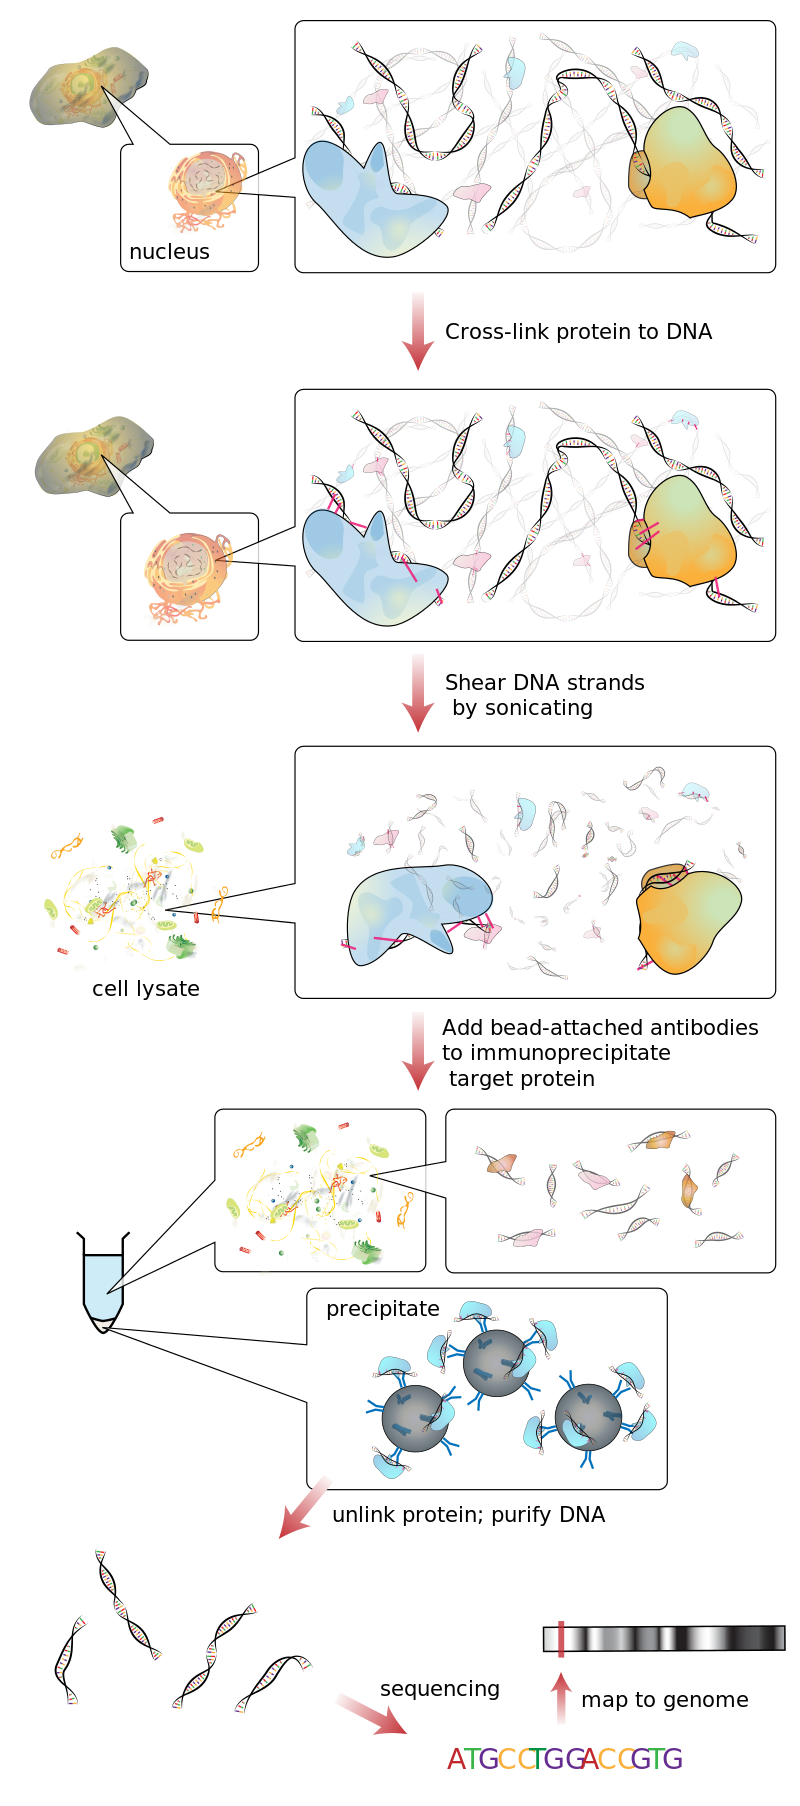
\includegraphics[width = 0.6\textwidth]{../images/ChIP-seq_workflow.png}
\caption{An overview of ChIP-seq. Figure courtesy Jkwchui, Wikimedia Commons user.}
\label{fig:ChIP-seq_workflow}
\end{figure}

If you would like a different explanation of  may also like to check out the following excellent video on identifying genes regulated by a transcription factor. This video was produced by students in the 2020 PreCollege Program in Computational Biology at Carnegie Mellon. The presenters won an award from their peers for their work, and for good reason! http://www.cbd.cmu.edu/education/pre-college-program-in-computational-biology\\

\begin{qbox}[%  
How do you think that researchers could determine whether a transcription factor activates or inhibits a given gene?
]\end{qbox} 


\FloatBarrier
\phantomsection
\subsection{Organizing transcription factor information}

As a result of techniques like ChIP-seq, researchers have learned a great deal about which transcription factors regulate which genes. But what can we do with this information?

We would like to organize the relationships between transcription factors and the genes they regulate in a way that will help us identify patterns in these relationships. In the next section, we will see that consolidating gene regulatory information into a \textit{network} will allow us to infer how cells have evolved to quickly change the expression of their genes in response to a dynamic environment.


\FloatBarrier
\phantomsection

\section{Transcription Factor Networks}
\label{sec:transcription_factor_networks}
\phantomsection

\subsection{The transcription factor network of \textit{E. coli}}

Once we know which genes each transcription factor regulates, we can consolidate this information into a \textdef{transcription factor network}{transcription factor network}{FILL IN}. The nodes in the network represent an organism's proteins, and we connect \textvar{X} to \textvar{Y} with an edge if \textvar{X} is a transcription factor that regulates the expression of protein \textvar{Y}. These edges are one-way connections; any node can have an edge leading into it, but only a transcription factor can have an edge leaving it.

\autoref{fig:e_coli_tf_network} shows a portion of the transcription factor network for \textit{Escherichia coli}, the workhorse model organism of bacterial studies. Even though \textit{E. coli} is a bacterium, we will be able to draw powerful conclusions about gene regulation from its transcription factor network. The true network, the sum of over two decades of biological research, consists of thousands of genes and around 300 transcription factors. Because of the size of this network, it forms what computational biologists affectionally call a ``hairball'', or a network with so many connections that it is functionally impossible to analyze visually. For this reason, we will need to use computational approaches to study our hairball.

Note that the edges in the \textit{E. coli} transcription factor network below are colored red or green. An edge connecting \textvar{X} to \textvar{Y} is colored green if \textvar{X} upregulates \textvar{Y}, and it is colored red if \textvar{X} downregulates \textvar{Y}. (Alternatively, we could label the edges with a ``+'' or ``-''.)

\begin{figure}[h]
\centering
\mySfFamily
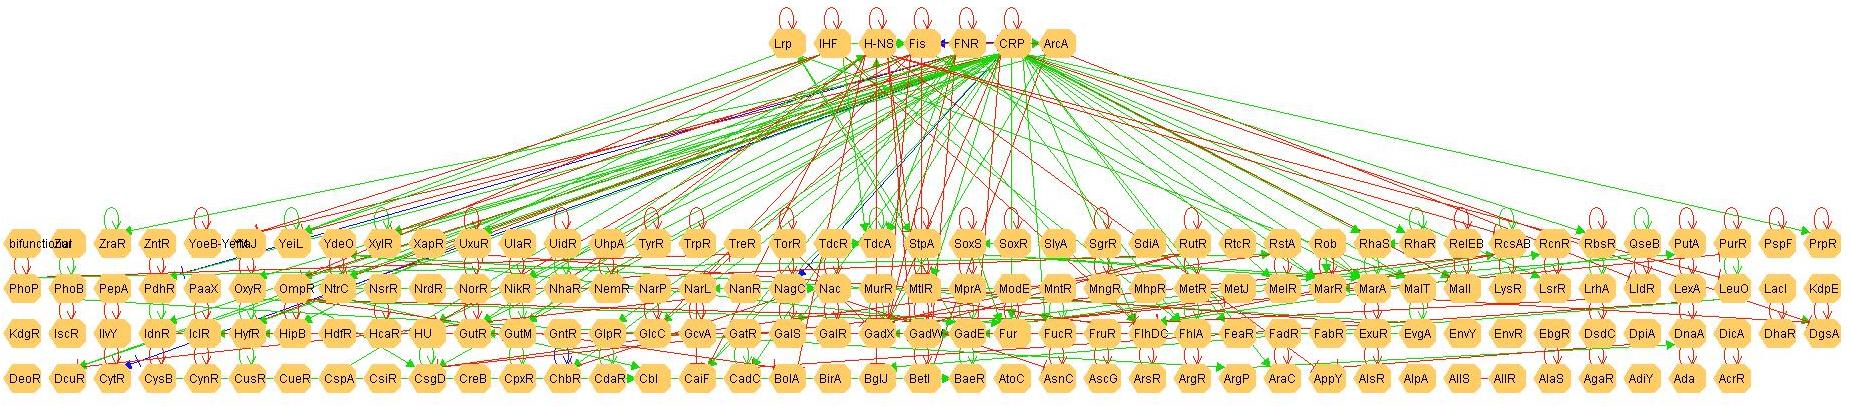
\includegraphics[width = 0.85\textwidth]{../images/e_coli_tf_network.jpeg}
\caption{A subset of the \textit{E. coli} transcription factor network. An edge from \textvar{X} to \textvar{Y} denotes that \textvar{X} is a transcription factor that regulates \textvar{Y}. Edges corresponding to upregulation are colored green, and edges corresponding to downregulation are colored red.}
\label{fig:e_coli_tf_network}
\end{figure}

\begin{qbox}[% 
Select the expanded view of the transcription factor network in \autoref{fig:e_coli_tf_network}. Do you notice anything interesting about this network?
]\end{qbox} 

\FloatBarrier
\phantomsection
\subsection{(Feedback) loops in the transcription factor network}

You may have noticed that the \textit{E. coli} transcription factor network seems to have surprisingly many \textdef{loops}{loops}{FILL IN}, or edges that connect a node to itself. It is worth pausing for a moment to consider the implications of a loop in a transcription factor network. What does it mean for a transcription factor to regulate itself?

A transcription factor is a protein, which means that because of the Central Dogma of Molecular Biology, the transcription factor is produced as the result of transcription and translation of a gene appearing in an organism's DNA. In \textdef{autoregulation}{autoregulation}{FILL IN}, illustrated in \autoref{fig:autoregulation_example}, the transcription factor protein then binds to the DNA in the upstream region of the gene encoding the \textit{same} transcription factor. This type of \textdef{feedback}{feedback}{FILL IN} is a beautiful and surprising feature of a simple biological system.\\

\begin{figure}[h]
\centering
\mySfFamily
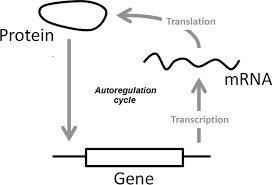
\includegraphics[width = 0.6\textwidth]{../images/autoregulation_example.png}
\caption{A simplified illustration of autoregulation. ``Protein'' labels the transcription factor binding factor protein, which binds to the DNA encoding this transcription factor, labeled by ``Gene''.}
\label{fig:autoregulation_example}
\end{figure}

Transcription factor autoregulation leads us to ask two questions. First, how can we justify that a transcription factor network has ``surprisingly many'' loops? And second, if autoregulation is so common, then why would a transcription factor have evolved to regulate its own transcription? We will address these questions in each of the next two sections.


\FloatBarrier
\phantomsection

\section{Gene Autoregulation is Surprisingly Frequent}
\label{sec:gene_autoregulation_is_surprisingly_frequent}
\phantomsection

\subsection{Using randomness to determine statistical significance}

In the previous section, we introduced the transcription factor network, in which a protein \textvar{X} is connected to a protein \textvar{Y} if \textvar{X} is a transcription factor that regulates the production of \textvar{Y}. We also saw that in the \textit{E. coli} transcription factor network, there seemed to be a large number of loops, or edges connecting some transcription factor \textvar{X} to itself, and which indicate the autoregulation of \textvar{X}.

In the introduction, we briefly referenced the notion of a network motif, a structure occurring often throughout a network. Our assertion is that the loop is a motif in the transcription factor network; how can we defend this claim?

To argue that a loop is indeed a motif in the \textit{E. coli} transcription factor network, we will apply a paradigm that occurs throughout computational biology (and science in general) when determining whether an observation is statistically significant. We will compare our observation against a  \textit{randomly generated} dataset. Without getting into the statistical details, if an observation is frequent in a real dataset, and rare in a random dataset, then it is likely to be statistically significant. Randomness saves the day again!\\

\begin{note}[% 
A seminal biological example of this paradigm is the search tool BLAST, which allows researchers to compare a sequence query against a database (e.g., comparing the DNA sequence of a newly sequenced gene against a collection of many known proteins). Once BLAST finds a ``hit'', or a location in the database where the query occurs with minimal modifications, it asks, ``What is the \textit{probability} that we would find a hit of the same quality of the query against a randomly generated 'decoy' database?'' If this probability is low, then we can feel confident that the hit is statistically significant.
]\end{note} 

\fudgespace

 \begin{qbox}[% 
 How can we apply this paradigm of a randomly generated dataset to determine whether a transcription factor network contains a significant number of loops?
 ]\end{qbox} 
 
\FloatBarrier
\phantomsection
\subsection{Comparing a real transcription factor network against a random network}

To determine whether the number of loops in the transcription factor network of \textit{E. coli} is statistically significant, we will compare this number of loops against the expected number of loops we would find in a randomly generated transcription factor network. If the number of loops in the real network is much higher than the number of loops in the random network, then we have strong evidence that some selective force is causing gene autoregulation.

There are multiple ways to generate a random network, but we will use an approach developed by Edgar Gilbert in 1959. Given an integer \textvar{n} and a probability \textvar{p} (between 0 and 1), we form \textvar{n} nodes. Then, for every possible pair of nodes \textvar{X} and \textvar{Y}, we connect \textvar{X} to \textvar{Y} via a directed edge with probability \textvar{p}; that is, we simulate the process of flipping a weighted coin that has probability \textvar{p} of coming up ``heads''.\\

\begin{note}[% 
 If you are interested in the technical details of how this can be simulated computationally, see https://compeau.cbd.cmu.edu/programming-for-lovers/chapter-2-forecasting-a-presidential-election-with-monte-carlo-simulation/
]\end{note}

\fudgespace

\begin{qbox}[% 
What should \textvar{n} and \textvar{p} be if we are generating a random network to compare against the \textit{E. coli} transcription factor network?
]\end{qbox} 

The full \textit{E. coli} transcription factor network contains thousands of genes, most of which are not transcription factors. As a result, the approach described above may form a random network that connects non-transcription factors to other nodes, which we should avoid.

Instead, we will focus on the network comprising only those \textit{E. coli} transcription factors that regulate each other. This network has 197 nodes and 477 edges, and so we will begin by forming a random network with $\textvar{n} = 197$ nodes.

We then select \textvar{p} to ensure that our random network will on average have 477 edges. To do so, we note that there are $\textvar{n}^2$ pairs of nodes that could have an edge connecting them (\textvar{n} choices for the starting node and \textvar{n} for the ending node). If we were to set \textvar{p} equal to $1/n^2$, then we would expect on average only to see a single edge in the random network. We therefore scale this value by 477 and set \textvar{p} equal to $477n/2 \approx 0.0123$ so that we will see, on average, 477 edges in our random network.

In the following tutorial, we write some code to count the number of loops in the real \textit{E. coli} transcription factor network. We then build a random network and compare the number of loops found in this network against the number of loops in the real network.

\FloatBarrier
\phantomsection
\subsection{The negative autoregulation motif}

In a random network containing \textvar{n} nodes, the probability that a given edge is a loop is 1/\textvar{n}. Therefore, if the network has \textit{e} edges, then we would on average see \textit{e}/\textvar{n} loops in the network. In our case, \textvar{n} is 197, and \textit{e} is 477; therefore, on average, we will only see approximately $197/497 \approx 2.42$ loops in a random network. Yet the real \textit{E. coli} network of transcription factors that regulate each other contains 130 loops!

Furthermore, in a random network, we would expect about half of the edges correspond to activation, and the other half correspond to repression. But if you followed the preceding tutorial, then you know that of the 130 loops in the \textit{E. coli} network, 35 correspond to upregulation and 95 correspond to downregulation. If this observation were not significant, then you should not be surprised to flip a coin 130 times and see ``heads'' come up 95 times.

Not only is autoregulation an important feature of transcription factors, but these transcription factors tend to \textit{negatively} autoregulate. Why in the world would organisms have evolved the process of autoregulation only for a transcription factor to \textit{slow down} its own transcription? In the next section, we will begin to unravel the mystery.\\


\FloatBarrier
\phantomsection

\section{The Negative Autoregulation Motif}
\label{sec:the_negative_autoregulation_motif}
\phantomsection

\subsection{Hunting for a biological motivation for negative autoregulation}

Theodosius Dobzhansky famously wrote that ``nothing in biology makes sense except in the light of evolution.'' In the spirit of this quotation, there must be some evolutionary reason for the presence of the large number of negatively autoregulating \textit{E. coli} transcription factors that we identified in the section. We will use biological modeling to establish this justification.

Say that a transcription factor \textvar{X} regulates another transcription factor \textvar{Y}, and consider two cells. In both cells, \textvar{X} upregulates the transcription of \textvar{Y}, but in the second cell, \textvar{Y} also negatively autoregulates; see \autoref{fig:two_cells} for an illustration.

\begin{figure}[h]
\centering
\mySfFamily
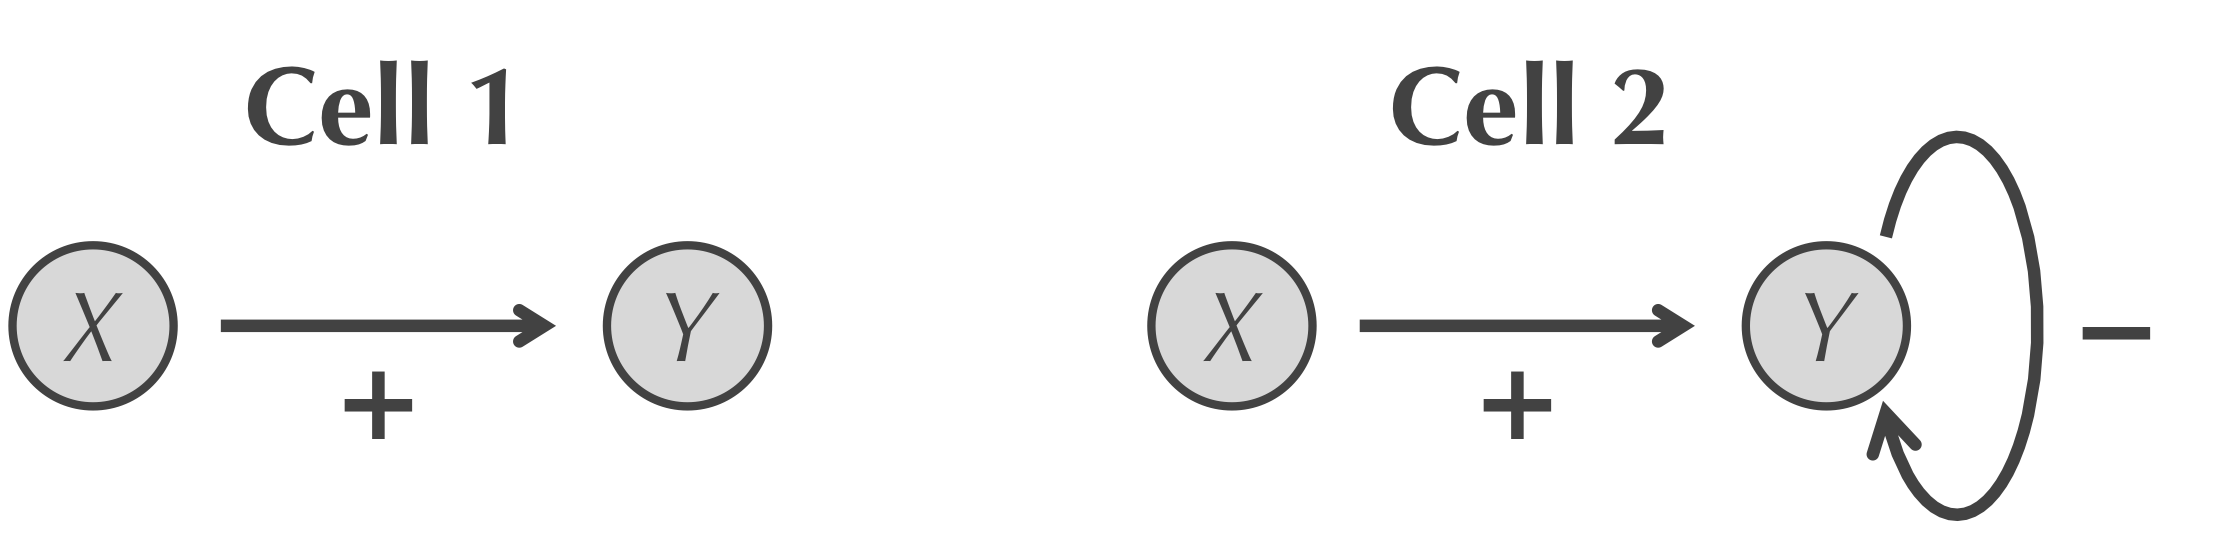
\includegraphics[width = 0.6\textwidth]{../images/two_cells.png}
\caption{The two cells that we wish to simulate. In the first cell (left), \textvar{X} only activates \textvar{Y}; in the second cell (right), \textvar{Y} also negatively autoregulates.}
\label{fig:two_cells}
\end{figure}

In this section, we will simulate a ``race'' to the \textdef{steady state}{steady state}{FILL IN}, or \textdef{equilibrium}{equilibrium}{FILL IN}, concentration of \textvar{Y} in the two cells. Our premise is that the cell that reaches the steady state faster can respond more quickly to its environment and is therefore more fit for survival.

\FloatBarrier
\phantomsection
\subsection{Simulating transcriptional regulation with a reaction-diffusion model}

In \autoref{chapter:turing}, we used a particle-based model to simulate a reaction-diffusion process. In this section, we will apply the same type of model, in which our ``particles'' are the two transcription factors \textvar{X} and \textvar{Y}.

We will begin with a model of the first cell, in which \textvar{X} activates \textvar{Y} but we do not have negative autoregulation of \textvar{Y}. To simulate \textvar{X} activating \textvar{Y}, we use the reaction $\textvar{X} \rightarrow \textvar{X} + \textvar{Y}$. In a given interval of time, there is a constant underlying probability related to the reaction rate that any given \textvar{X} particle will spontaneously form a new \textvar{Y} particle.

We should also account for the fact that proteins are \textit{degraded} over time by enzymes called proteases. The typical protein's concentration will be degraded by 20 to 40 percent in an hour, but transcription factors degrade even faster, only lasting a matter of minutes. Degradation may seem like a bug of cellular design, but it is a feature, as it allows the cell to remove a protein after increasing that protein's concentration in response to some environmental change.

To model the degradation of a protein, we add a ``kill'' reaction that removes \textvar{Y} particles at some rate. We will initialize our simulation with no \textvar{Y} particles and the \textvar{X} concentration at steady state, so that \textvar{X} is being produced at a rate that exactly balances its degradation rate, and we will therefore not need to add reactions to the model simulating the production or degradation of \textvar{X}.

To complete the model of the first cell, diffusion of the \textvar{X} and \textvar{Y} particles is not technically necessary because there is no reaction having more than one particle as a reactant. However, for the sake of biological correctness, we will allow both \textvar{X} and \textvar{Y} particles to diffuse through the system at the same rate.\\

\begin{qbox}[% 
What chemical reaction could be used to simulate the negative autoregulation of \textvar{Y}?
]\end{qbox} 

We now will simulate the second cell, which will inherit all of the reactions from the first cell (with the same reaction rates) while adding negative autoregulation of \textvar{Y}. We will do so using the reaction $2\textvar{Y} \rightarrow \textvar{Y}$. In other words, when two \textvar{Y} particles collide, there is some probability related to the reaction rate that one of the particles serves to remove the other, which mimics the process of a transcription factor turning off another copy of itself during negative autoregulation.

To recap, the simulations of both cells will include an initial concentration of \textvar{X} at steady state, diffusion of \textvar{X} and \textvar{Y}, removal of \textvar{Y}, and the reaction $\textvar{X} \rightarrow \textvar{X} + \textvar{Y}$. The second simulation, which includes negative autoregulation of \textvar{Y}, will add the reaction $2\textvar{Y} \rightarrow \textvar{Y}$. \tutorial[https://biologicalmodeling.org/motifs/tutorial_nar]\\

\begin{note}[% 
Even though we are using a particle-based model to mimic regulation, it is not attempting to replicate specific chemical reactions. In reality, gene regulation is a complicated chemical process that involves a great deal of molecular machinery. However, this is the purpose of the model, to strip away what is not relevant and retain the essence of what is being modeled.
]\end{note} 

\FloatBarrier
\phantomsection
\subsection{Ensuring a mathematically controlled comparison}

If you followed the previous tutorial, then you were likely disappointed in the second cell and its negative autoregulating transcription factor \textvar{Y}. \autoref{fig:nar_unequal_chart} shows a plot of the concentration of \textvar{Y} particles for the two simulations; the first cell is shown in red, and the second cell is shown in yellow.

\begin{figure}[h]
\centering
\mySfFamily
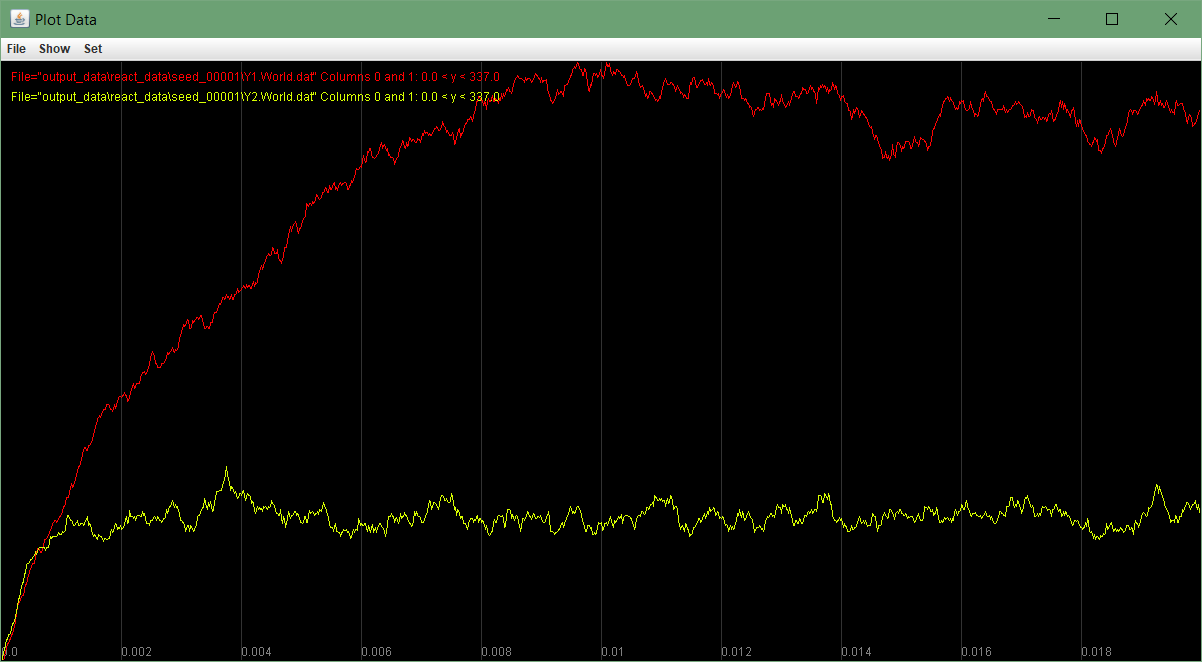
\includegraphics[width = 0.85\textwidth]{../images/nar_unequal_chart.png}
\caption{A comparison of the number of \textvar{Y} particles across two simulations. In the first cell (red), we only have upregulation of \textvar{Y} by \textvar{X}, whereas in the second cell (yellow), we keep all parameters fixed but add a reaction simulating negative autoregulation of \textvar{Y}.}
\label{fig:nar_unequal_chart}
\end{figure}

By allowing \textvar{Y} to slow its own transcription, we wound up with a simulation in which the final concentration of \textvar{Y} was \textit{lower}. It seems like we are back where we started!

The solution to our quandary is that the model we built was not a fair comparison between the two systems. In particular, the two simulations should be controlled so that they have approximately the \textit{same} steady state concentration of \textvar{Y}, since this concentration represents the cell's response to some stimulus. Ensuring this equal footing for the two simulations is called a \textdef{mathematically controlled comparison}{mathematically controlled comparison}{FILL IN}.\\

\begin{qbox}[% 
How can we change the parameters of our models to obtain a mathematically controlled comparison?
]\end{qbox} 

There are a number of parameters that we should keep constant across the two simulations because they are unrelated to regulation: the diffusion rates of \textvar{X} and \textvar{Y}, the number of initial particles \textvar{X} and \textvar{Y}, and the degradation rate of \textvar{Y}.

With these parameters fixed, the only way that the steady state concentration of \textvar{Y} can be the same in the two simulations is if we \textit{increase} the rate at which the reaction $\textvar{X} \rightarrow \textvar{X} + \textvar{Y}$ takes place in the simulation of the second cell. The following tutorial adjusts this rate parameter to ensure a mathematically controlled comparison.

\tutorial[https://biologicalmodeling.org/motifs/tutorial_nar_mathematically_controlled]

\FloatBarrier
\phantomsection
\subsection{An evolutionary basis for negative autoregulation}

\autoref{fig:nar_equal_chart} plots the number of \textvar{Y} particles for the two simulations on the same chart over time, with the rate of the $\textvar{X} \rightarrow \textvar{X} + \textvar{Y}$ reaction increased in the simulation involving negative autoregulation. Both  simulations now have approximately the same steady state concentration of \textvar{Y}. However, the second simulation reaches this concentration faster; that is, its \textdef{response time}{response time}{FILL IN} to the external stimulus causing an increase in the production of \textvar{Y} is shorter.\\

\begin{figure}[h]
\centering
\mySfFamily
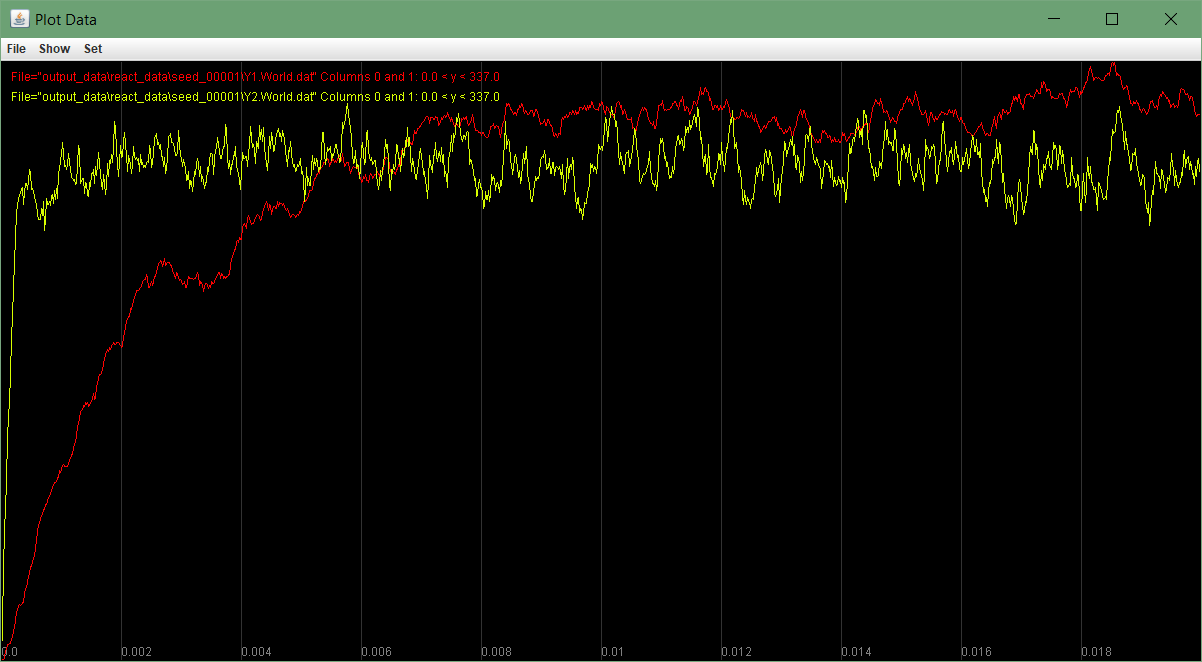
\includegraphics[width = 0.85\textwidth]{../images/nar_equal_chart.png}
\caption{A comparison of the concentration of \textvar{Y} particles across the same two simulations from \autoref{fig:nar_unequal_chart}. This time, in the second simulation (yellow), we increase the rate of the reaction $\textvar{X} \rightarrow \textvar{X} + \textvar{Y}$.  As a result, the two simulations have approximately the same steady state concentration of \textvar{Y}, and the simulation that includes negative autoregulation reaches steady state more quickly.}
\label{fig:nar_equal_chart}
\end{figure}

More importantly, this plot provides evidence of \textit{why} negative autoregulation may have evolved. The simulation involving negative autoregulation wins the ``race'' to a steady state concentration of \textvar{Y}, and so we can conclude that a cell in which this transcription factor is negatively autoregulated is more fit for survival than one that does not. Uri Alon has proposed an excellent analogy of a negatively autoregulating transcription factor as a sports car that has both a powerful engine (corresponding to the higher rate of the reaction producing \textvar{Y}) and sensitive brakes (corresponding to the negative autoregulation reaction slowing the production of \textvar{Y}).

In this section, we have seen that particle-based simulations can be powerful for justifying why a network motif is prevalent. What are some other commonly occurring network motifs in transcription factor networks? And what evolutionary purposes might they serve?\\


\FloatBarrier
\phantomsection

\section{The Feedforward Loop Motif}
\label{sec:the_feedforward_loop_motif}
\phantomsection

\subsection{Feedforward loops}

In the previous section, we saw that negative autoregulation can be used to lower the response time of a protein to an external stimulus. But the cell can only use negative autoregulation to respond quickly if the autoregulated protein is itself a transcription factor. Only about 300 out of 4,400 total \textit{E. coli} proteins are transcription factors. How can the cell speed up the manufacture of a protein if that protein is not a transcription factor?

The answer lies in another transcription factor network motif called the \textdef{feedforward loop}{feedforward loop}{FILL IN} (\textdef{FFL}{FFL}{FILL IN}). An FFL, shown in \autoref{fig:feed-forward_loop}, is a network substructure in which \textvar{X} is connected to both \textvar{Y} and \textvar{Z}, and \textvar{Y} is connected to \textvar{Z}. Calling the FFL motif a ``loop'' is a misnomer. Rather, it is a small structure in which there are two paths from \textvar{X} to \textvar{Z}; one via direct regulation of \textvar{Z} by \textvar{X}, and another with an intermediate transcription factor \textvar{Y}.\\

\begin{figure}[h]
\centering
\mySfFamily
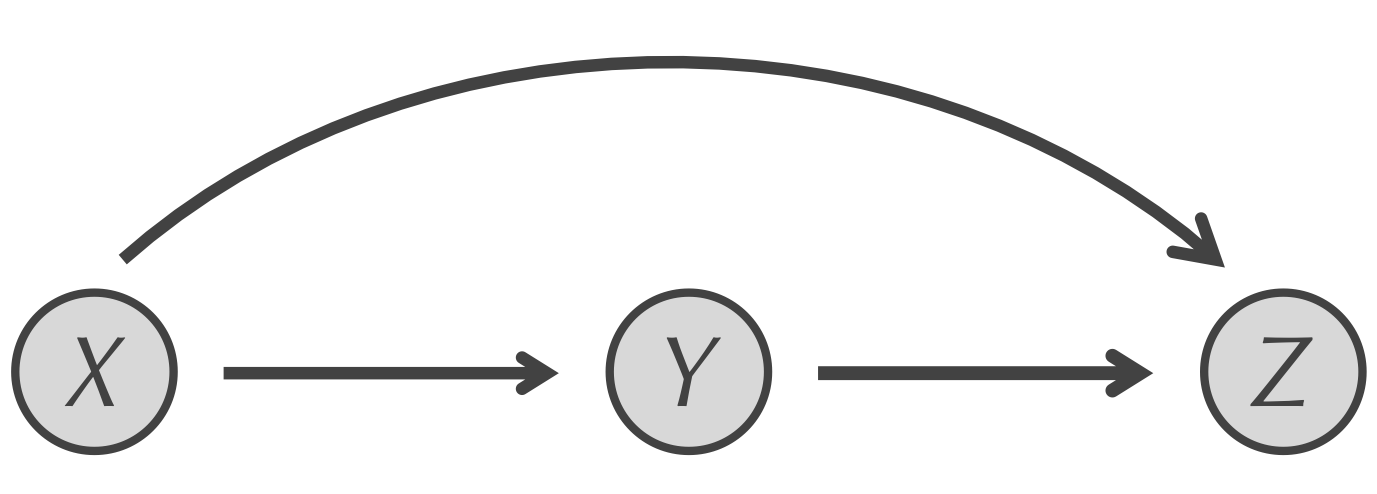
\includegraphics[width = 0.6\textwidth]{../images/feed-forward_loop.png}
\caption{The FFL motif. \textvar{X} regulates both \textvar{Y} and \textvar{Z}, and \textvar{Y} regulates \textvar{Z}.}
\label{fig:feed-forward_loop}
\end{figure}

Note that \textvar{X} and \textvar{Y} must be transcription factors because they have edges leading out from them, but \textvar{Z} does not have to be a transcription factor (and in fact typically is not). There are 42 FFLs in the transcription factor network of \textit{E. coli}; we leave the verification that this number is significant as an exercise at the end of the section.

Recall that every edge of a transcription factor network is assigned a sign based on whether the regulation represented by the edge corresponds to activation or repression, respectively. Accordingly, since an FFL involves three different regulation events, there are $2^3$ = 8 different types of FFLs.

Among the 42 total FFLs in the \textit{E. coli} transcription factor network, five of them have the structure below, in which the edges connecting \textvar{X} to \textvar{Y} and \textvar{X} to \textvar{Z} are assigned a ``+'' and the edge connecting \textvar{Y} to \textvar{Z} is assigned a ``-''. This specific form of the FFL motif is  called a \textdef{type-1 incoherent feedforward loop}{type-1 incoherent feedforward loop}{FILL IN}. This form of the FFL will be our focus for the rest of the section.\\

\begin{qbox}[% 
How could we simulate a feedforward loop with a particle-based reaction-diffusion model akin to the simulation that we used for negative autoregulation? What would we compare this simulation against?
]\end{qbox} 

\begin{figure}[h]
\centering
\mySfFamily
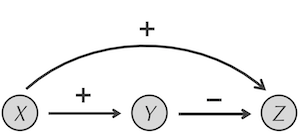
\includegraphics[width = 0.6\textwidth]{../images/type-1_incoherent_feed-forward_loop.png}
\caption{The incoherent feed-forward loop network motif. Note that \textvar{X} upregulates \textvar{Y} and \textvar{Z}, while \textvar{Y} downregulates \textvar{Z}.}
\label{fig:type-1_incoherent_feed-forward_loop}
\end{figure}

\FloatBarrier
\phantomsection
\subsection{Modeling a type-1 incoherent feedforward loop}

As we did in the last section, we will run two simulations. In the first, we will have a simple activation of \textvar{Z} by \textvar{X}, meaning that we will assume \textvar{X} is at its steady state concentration and that \textvar{Z} is produced by the reaction $\textvar{X} \rightarrow \textvar{X} + \textvar{Z}$ and removed by a degradation reaction.

The second simulation will include both of these reactions, but we will also have the reaction $\textvar{X} \rightarrow \textvar{X} + \textvar{Y}$ to model the activation of \textvar{Y} by \textvar{X}, along with the new reaction $\textvar{Y} + \textvar{Z} \rightarrow \textvar{Y}$ to model the repression of \textvar{Z} by \textvar{Y}. Because \textvar{Y} and \textvar{Z} are being produced from a reaction, we will also have degradation reactions for \textvar{Y} and \textvar{Z}. For the sake of fairness, we will use the same kill rates for both \textvar{Y} and \textvar{Z}.

Furthermore, to obtain a mathematically controlled comparison, the reaction $\textvar{X} \rightarrow \textvar{X} + \textvar{Z}$ should have a higher rate in the second simulation modeling the FFL. If we do not raise the rate of this reaction, then the repression of \textvar{Z} by \textvar{Y} will cause the steady state concentration of \textvar{Z} to be lower in the second simulation.

If you are feeling adventurous, then you may like to adapt the code from the previous tutorial to run the above two simulations and tweak the rate of the $\textvar{X} \rightarrow \textvar{X} + \textvar{Z}$ reaction to see if you can obtain the same steady state concentration of \textvar{Z} in the two simulations. We also provide the following tutorial guiding you through setting up these simulations, which we will interpret in the next section.

\tutorial[https://biologicalmodeling.org/motifs/tutorial_feed]

\FloatBarrier
\phantomsection
\subsection{Why feedforward loops speed up response times}

\autoref{fig:ffl_chart} shows a plot visualizing the amount of \textvar{Z} across the two simulations. As with negative autoregulation, the type-1 incoherent FFL allows the cell to ramp up production of a gene \textvar{Z} much faster than it would under simple regulation.\\

\begin{figure}[h]
\centering
\mySfFamily
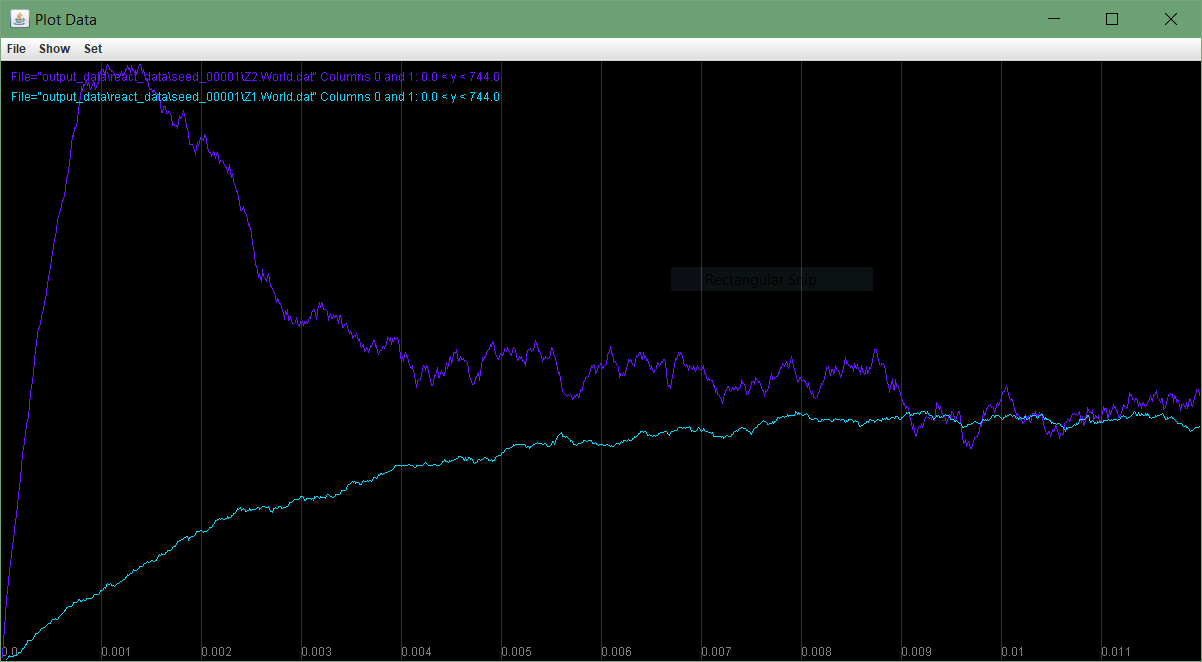
\includegraphics[width = 0.85\textwidth]{../images/ffl_chart.png}
\caption{The concentration of \textvar{Z} in the two simulations. Simple activation of \textvar{Z} by \textvar{X} is shown in blue, and the type-1 incoherent FFL is shown in purple.}
\label{fig:ffl_chart}
\end{figure}

However, you will note a slightly different pattern to the growth of \textvar{Z} than we saw under negative autoregulation. In negative autoregulation, the concentration of the protein approached steady state from below. In the case of the FFL, the concentration of \textvar{Z} grows so quickly that it passes its eventual steady state concentration and then returns to this steady state from above.

We can interpret from the model why the FFL allows for a fast response time as well as why it initially passes the steady state concentration. At the start of the simulation, \textvar{Z} is activated by \textvar{X} very quickly. \textvar{X} regulates the production of \textvar{Y} as well, but at a lower rate than the regulation of \textvar{Z} because \textvar{Y} only has its own degradation to slow this process. Therefore, more \textvar{Z} is initially produced than \textvar{Y}, which causes the concentration of \textvar{Z} to shoot past its eventual steady state.

The more \textvar{Y} we have, and the more \textvar{Z} that we have, the more often the repression reaction $\textvar{Y} + \textvar{Z} \rightarrow \textvar{Y}$ will occur. Because the concentrations of both \textvar{Y} and \textvar{Z} increase over time, this reaction serves as the ``brakes'' for the concentration of \textvar{Z}. These brakes need to be very powerful, meaning that the rate of the reaction $\textvar{Y} + \textvar{Z} \rightarrow \textvar{Y}$ needs to be very high, to decrease the concentration of \textvar{Z} to its steady state.

\FloatBarrier
\phantomsection
\subsection{Damped oscillations give us hope of building a biological oscillator}

Unlike negative autoregulation of a single transcription factor, the FFL requires \textit{two} separate transcription factors working together to increase the production of our target gene. This higher evolutionary cost of implementation may help account for why FFLs are more rare as a network motif than loops.

We only considered one of the eight types of FFL in this section. You might wonder whether any of the other seven FFLs serve as network motifs.  For example, what happens if \textvar{X} activates \textvar{Z}, \textvar{X} represses \textvar{Y}, and \textvar{Y} activates \textvar{Z}? We will explore these additional FFL motifs in the exercises at the end of the section.

Finally, recall that in our FFL model, the concentration of \textvar{Z} increased dramatically before decreasing to the steady state. \autoref{fig:ffl_chart} is reminiscent of a \textdef{damped oscillation}{damped oscillation}{FILL IN} process like the one in \autoref{fig:damped_oscillator}, in which the concentration of a particle oscillates above and below a steady state, while the amplitude of the wave gets smaller and smaller. Is it possible for a network motif to produce more of a true ``wave'' without dampening?\\

\begin{figure}[h]
\centering
\mySfFamily
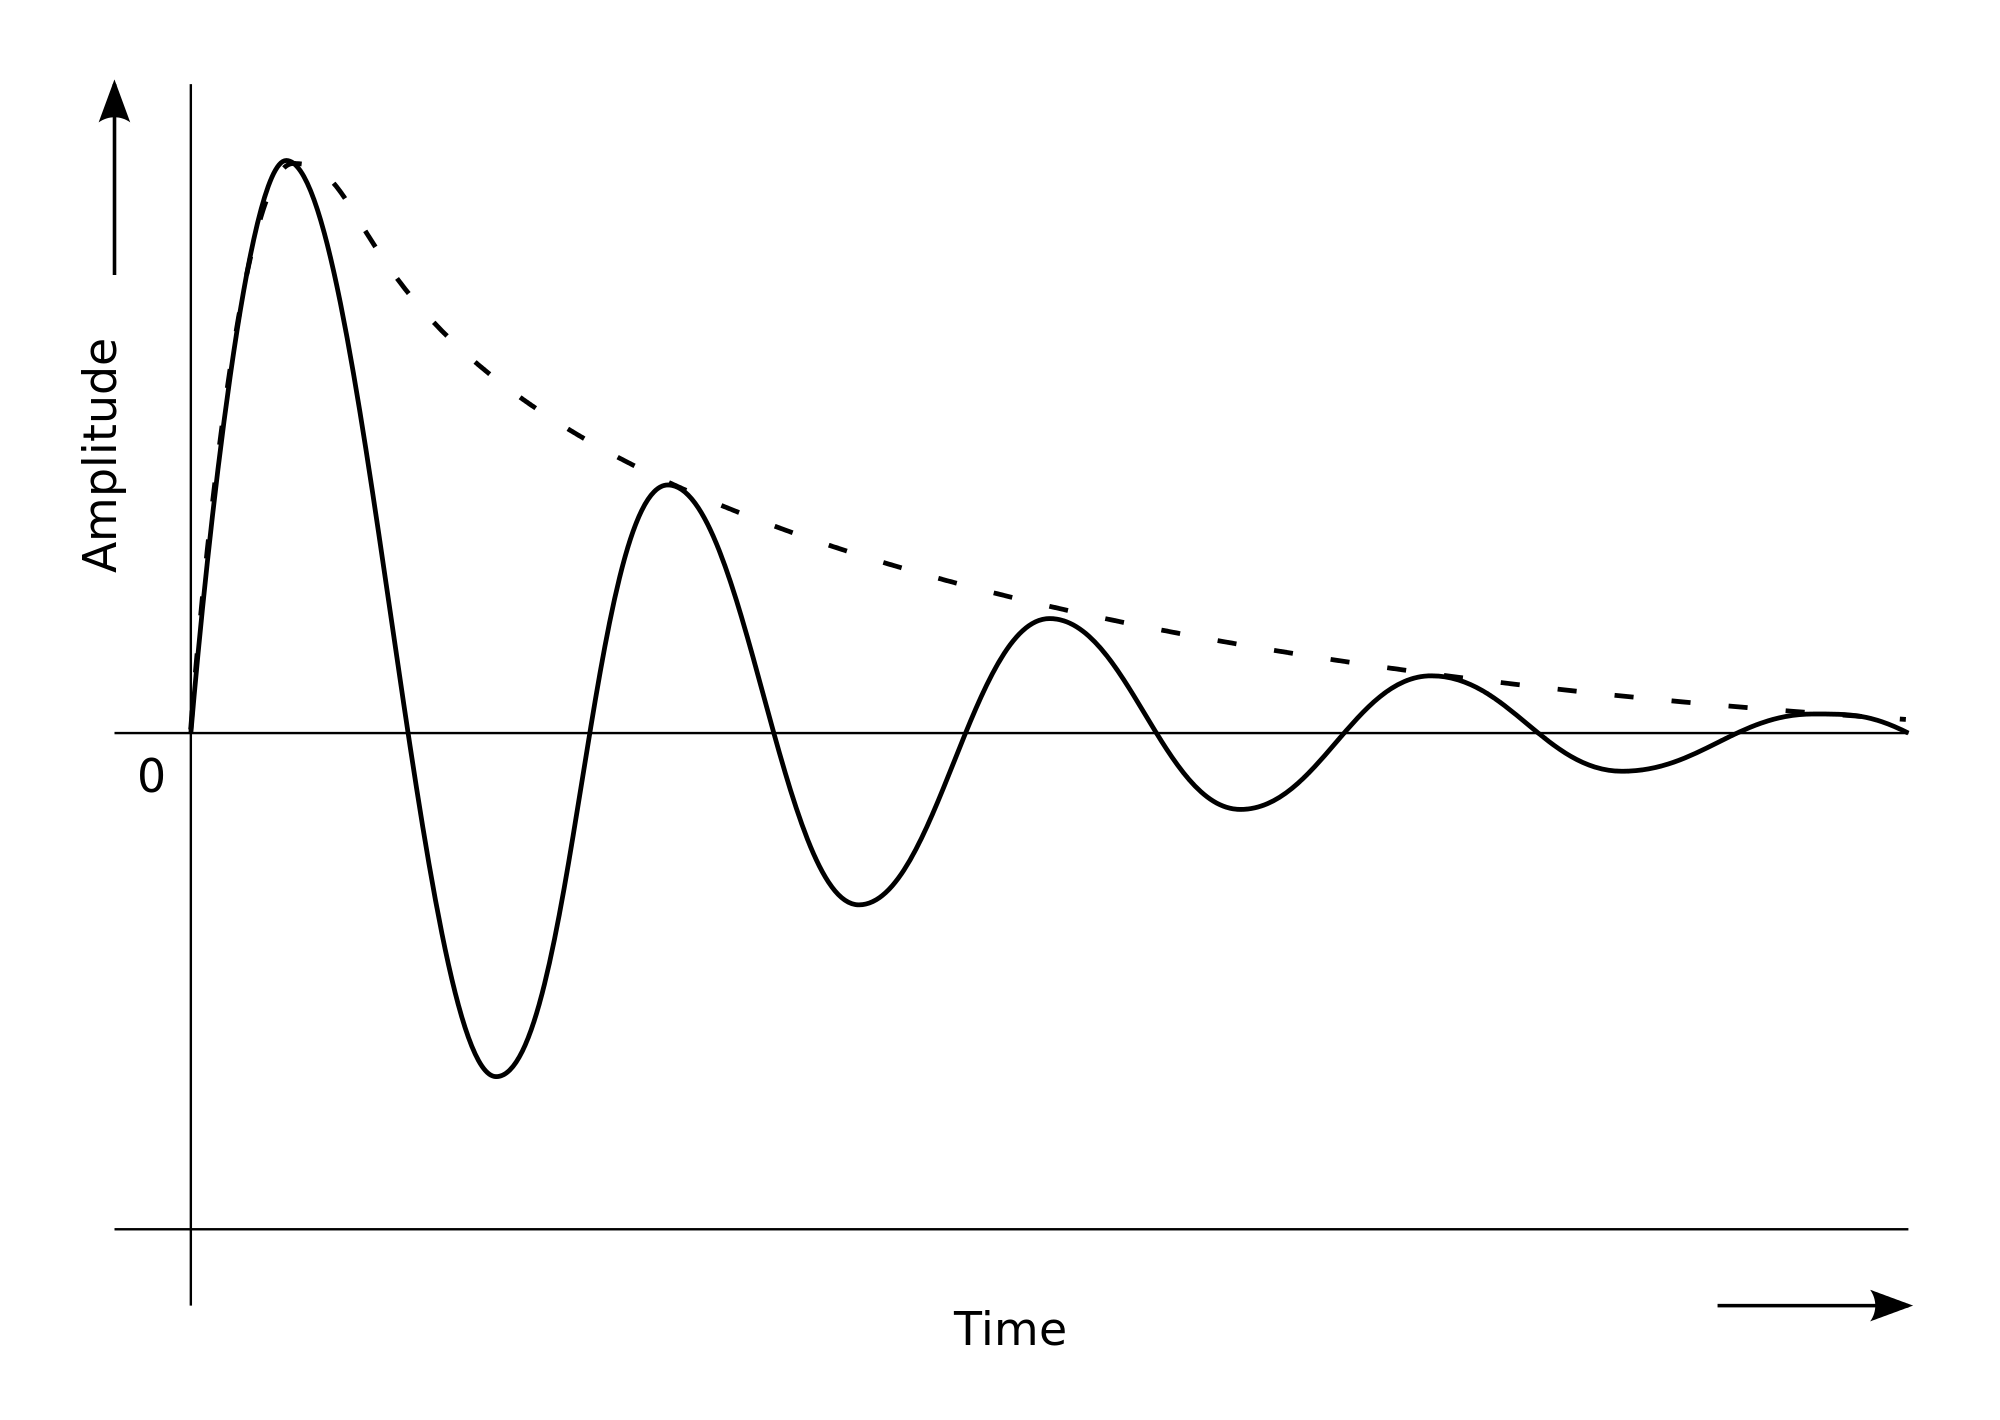
\includegraphics[width = 0.6\textwidth]{../images/damped_oscillator.png}
\caption{In a damped oscillation, the value of some variable (shown on the y-axis) oscillates back and forth around an asymptotic value while the amplitude decreases over time.}
\label{fig:damped_oscillator}
\end{figure}


\FloatBarrier
\phantomsection

\section{Biological Oscillators}
\label{sec:biological_oscillators}
\phantomsection

\subsection{Oscillators are everywhere in nature}

Even if placed in a bunker, humans will maintain a roughly 24-hour cycle of sleep and wakefulness. This \textdef{circadian rhythm}{circadian rhythm}{FILL IN} is present throughout living things, including plants and even cyanobacteria.

Life processes that oscillate over time are not confined to circadian rhythms. You may feel like you have control over when you go to bed, but your heart and respiratory system both follow subconscious cyclical rhythms, and your cells are governed by a strict cell cycle as they grow and divide.

We might guess from what we have learned in this section that cyclical biological rhythms must be governed by simple rules. However, the question remains as to what these rules are and how they can correctly execute oscillations over and over, throughout an organism's life.

Researchers have identified many network motifs that facilitate oscillation, some of which are very complicated and include many components. In this section, we will focus on a simple three-component oscillator motif called a \textdef{repressilator}{repressilator}{FILL IN}.

\FloatBarrier
\phantomsection
\subsection{The repressilator: a synthetic biological oscillator}

The repressilator motif is shown in \autoref{fig:repressilator}. In this motif, all three proteins are transcription factors, and they form a cycle in which \textvar{X} represses \textvar{Y}, \textvar{Y} represses \textvar{Z}, and \textvar{Z} represses \textvar{X}. The repressilator clearly forms a feedback loop, but nothing \textit{a priori} about this motif would indicate that it would lead to oscillation.\\

\begin{figure}[h]
\centering
\mySfFamily
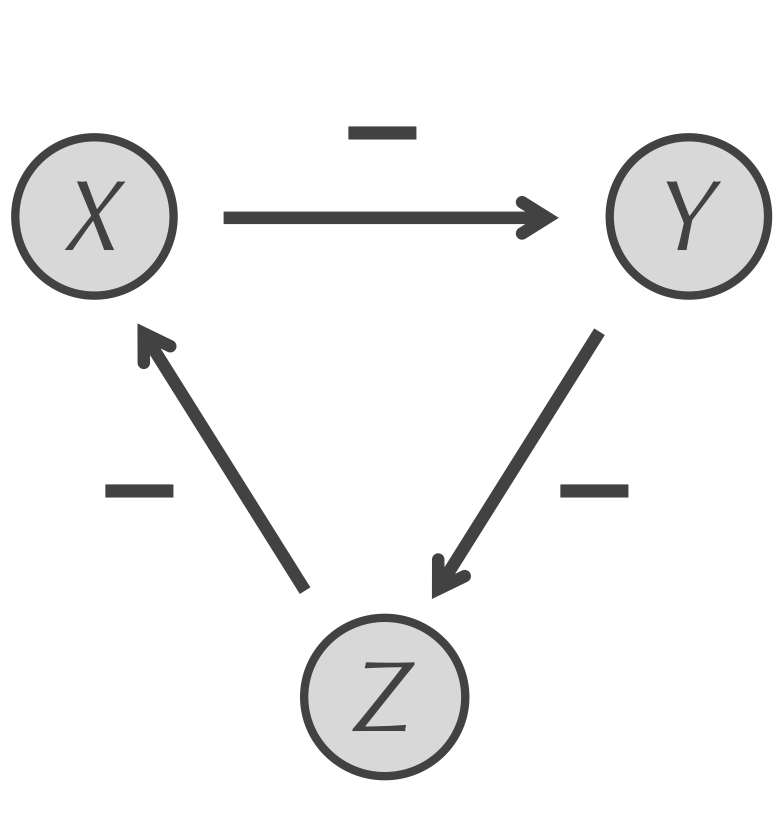
\includegraphics[width = 0.4\textwidth]{../images/repressilator.png}
\caption{The repressilator motif for three particles \textvar{X}, \textvar{Y}, and \textvar{Z}. \textvar{X} represses \textvar{Y}, which represses \textvar{Z}, which in turn represses \textvar{X}, forming a feedback loop.}
\label{fig:repressilator}
\end{figure}

\begin{qbox}[% 
Try to devise a reaction-diffusion model representing the repressilator.
]\end{qbox} 

To build a reaction-diffusion model accompanying the repressilator, we start with a quantity of \textvar{X} particles, and no \textvar{Y} or \textvar{Z} particles. We assume that all three particles diffuse at the same rate and degrade at the same rate.

Furthermore, we assume that all three particles are produced as the result of an activation process by some other transcription factor(s), which we assume happens at the same rate. We will use a \textdef{hidden particle}{hidden particle}{FILL IN} \textvar{I} that serves to activate the three visible particles via the three reactions $\textvar{I} \rightarrow \textvar{I} + \textvar{X}$, $\textvar{I} \rightarrow \textvar{I} + \textvar{Y}$, and $\textvar{I} \rightarrow \textvar{I} + \textvar{Z}$, all taking place at the same rate.

In the [previous section](feedforward) on the feed-forward loop, we saw that we can use the reaction $\textvar{X} + \textvar{Y} \rightarrow \textvar{X}$ to model the repression of \textvar{Y} by \textvar{X}. To complete the repressilator model, we will add the two reactions $\textvar{Y} + \textvar{Z} \rightarrow \textvar{Y}$ and $\textvar{Z} + \textvar{X} \rightarrow \textvar{Z}$, having the same rate as the reaction $\textvar{X} + \textvar{Y} \rightarrow \textvar{X}$.

If you followed our previous tutorials, then you may feel comfortable taking off the training wheels and implementing the repressilator with your own reaction-diffusion model, which we cover in the following tutorial.

\tutorial[https://biologicalmodeling.org/motifs/tutorial_oscillators]

\FloatBarrier
\phantomsection
\subsection{Interpreting the repressilator's oscillations}

\autoref{fig:repressilator_chart} shows a plot of the concentration of \textvar{X}, \textvar{Y}, and \textvar{Z} particles from our repressilator simulation. The system shows clear oscillatory behavior, with the concentrations of \textvar{X}, \textvar{Y}, and \textvar{Z} taking turns being at high concentration.\\

\begin{qbox}[% 
Why do you think that the repressilator motif leads to this pattern of oscillations?
]\end{qbox} 

\begin{figure}[h]
\centering
\mySfFamily
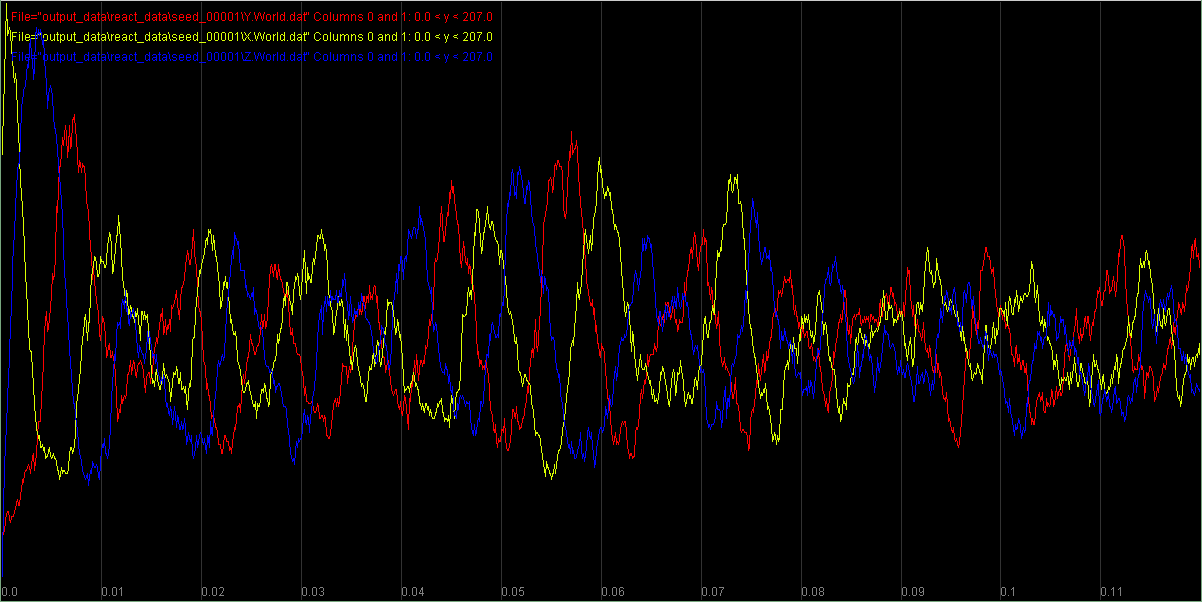
\includegraphics[width = 0.85\textwidth]{../images/repressilator_chart.png}
\caption{Modeling the repressilator's concentration of particles. \textvar{X} is shown in yellow, \textvar{Y} is shown in red, and \textvar{Z} is shown in blue}
\label{fig:repressilator_chart}
\end{figure}

Because the concentration of \textvar{X} starts out high, with no \textvar{Y} or \textvar{Z} present, the concentration of \textvar{X} briefly increases because its rate of production exceeds its rate of degradation. Because no \textvar{Y} or \textvar{Z} particles are present, there are none to degrade, and the concentrations of these particles start increasing as well.

As the concentration of \textvar{Z} rises, the repression reaction $\textvar{Z} + \textvar{X} \rightarrow \textvar{Z}$ occurs often enough for the rate of removal of \textvar{X} to equal and exceed its rate of production, accounting for the first peak in \autoref{fig:repressilator_chart}. Furthermore, because the concentration of \textvar{X} particles begins high, the repression reaction $\textvar{X} + \textvar{Y} \rightarrow \textvar{X}$ prevents the number of \textvar{Y} particles from growing initially.

In summary, after an initial rise, the concentration of \textvar{X} plummets, with the concentration of \textvar{Z} rising up to replace it. The concentration of \textvar{Y} increases, but at a slower rate than that of \textvar{Z}. This situation is shown by the second (blue) peak in \autoref{fig:repressilator_chart}.

As a result, \textvar{Z} and \textvar{X} have switched roles. Because there is a high concentration of \textvar{Z}, and the concentration of \textvar{Y} is increasing, the reaction $\textvar{Y} + \textvar{Z} \rightarrow \textvar{Y}$ will be frequent and reduce the concentration of \textvar{Z}. Furthermore, because the concentration of \textvar{X} has decreased, and the concentration of \textvar{Y} is still relatively low, the reaction $\textvar{X} + \textvar{Y} \rightarrow \textvar{X}$ will occur less often, allowing the concentration of \textvar{Y} to continue to rise. Eventually, the decrease in \textvar{Z} and the increase in \textvar{Y} will account for the third (red) peak in \autoref{fig:repressilator_chart}.

At this point, the reaction $\textvar{X} + \textvar{Y} \rightarrow \textvar{X}$ will suppress the concentration of \textvar{Y}. Because the concentration of \textvar{X} and \textvar{Z} are both lower than the concentration of \textvar{Z}, the reaction $\textvar{Z} + \textvar{X} \rightarrow \textvar{Z}$ will not greatly influence the concentration of \textvar{X}, which will rise to meet the following concentration of \textvar{Y}, and we have returned to our original situation, at which point the cycle will begin again.

\FloatBarrier
\phantomsection
\subsection{The power of noise}

Take another look at the oscillations of the repressilator in \autoref{fig:repressilator_chart}. You will notice that the concentrations zigzag as they travel up or down, and that they peak at slightly different levels each time.

This noise in the repressilator's oscillations is due to random variation as the particles bounce around due to diffusion. The repression reactions require two particles to collide in order for the reaction to take place. Due to random chance, these collisions may occur more or less often than expected because of random chance. Much of this noise is due to low sample size: we have around 150 molecules at each peak in the \autoref{fig:repressilator_chart}, but a given cell may have on the order of 1,000 to 10,000 molecules of a single protein.

Yet the noise that appears in the repressilator's oscillations is a feature, not a bug. As we have discussed previously, the cell's molecular interactions are inherently random. So if we see oscillations in a simulation that includes noise arising from random chance, then we can be confident that this simulation is \textit{robust} to a certain amount of variation.

In this section's conclusion, we will further explore the concept of robustness as it pertains to the repressilator. What happens if our simulation experiences a much greater disturbance to the concentration of one of the particles?  Will it still be able to recover and return to the same oscillatory pattern?\\

\FloatBarrier
\phantomsection

\section{Conclusion: The Robustness of Biological Oscillators}
\label{sec:biological_oscillators_must_be_robust}
\phantomsection

\subsection{Biological oscillators must be robust}

Nothing exemplifies the need for robustness in biological systems better than oscillators. If your heart skips a beat when you are watching a horror movie, then it should return quickly to its natural rhythm. When you hold your breath to dive underwater, your normal breathing resumes at the surface. And regardless of what functions your cells perform or what disturbances they find in their environment, they should be able to maintain a normal cell cycle.

An excellent illustration of oscillator robustness is the body's ability to handle jet lag. There is no apparent reason why humans would have evolved to be resilient to flying halfway around the world. And yet our circadian clock is so resilient that after a few days of fatigue and crankiness, our circadian clock returns to a normal daily cycle.

In the previous section, we saw that the repressilator, a three-element motif, can exhibit oscillations even in a noisy environment of randomly moving particles. The repressilator's resilience makes us wonder how well the repressilator can respond to a disturbance in the concentrations of its particles.

\FloatBarrier
\phantomsection
\subsection{A coarse-grained repressilator model}

As we saw in \autoref{chapter:turing} with our work on Turing patterns, tracking the movements of many individual particles led to a slow simulation that did not scale well given more particles or reactions. This observation led us to devise a coarse-grained reaction-diffusion model that was still able to produce Turing patterns. We used a cellular automaton because the concentrations of particles varied in different locations and were diffusing at different rates.

We would like to devise a coarse-grained model of the repressilator. However, the particles diffuse at the same rate and are \textit{uniform} across the simulation, and so there is no need to track concentrations in individual locations. As a result, we will need a simulation that assumes that the particles are \textdef{well-mixed}{well-mixed}{FILL IN}.

For example, say that we are modeling a degradation reaction. If we start with 10,000 \textvar{X} particles, then after a single time step, we will simply multiply the number of \textvar{X} particles by (1-\textit{k}), where \textit{k} is a parameter related to the rate of the degradation reaction.

As for a repression reaction like $\textvar{X} + \textvar{Y} \rightarrow \textvar{X}$, we can update the concentration of \textvar{Y} particles by subtracting some factor \textit{r} times the current concentration of \textvar{Y} particles. This factor should be directly correlated with the current concentrations of both \textvar{X} and \textvar{Y}.

We will discuss the technical details behind our well-mixed model in the next section. In the meantime, we would like to see what happens when we make a major disturbance to the concentration of one of the particles in the well-mixed model to see whether the particle concentrations resume their oscillations. 

\tutorial[https://biologicalmodeling.org/motifs/tutorial_perturb]

\FloatBarrier
\phantomsection
\subsection{The repressilator is robust to disturbance}

\autoref{fig:nf_sim_interrupted_chart} shows a plot of concentrations of each particle in our well-mixed simulation of the repressilator.  Midway through this simulation, we greatly increase the concentration of \textvar{Y} particles.

\begin{figure}[h]
\centering
\mySfFamily
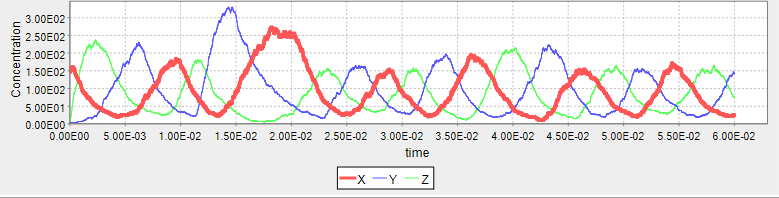
\includegraphics[width = 0.85\textwidth]{../images/nf_sim_interrupted_chart.png}
\caption{A plot of particle concentrations in the well-mixed repressilator model over time. Adding a significant number of \textvar{Y} particles to our simulation (the second blue peak) produces little ultimate disturbance to the concentrations of the three particles, which return to normal oscillations within a single cycle.}
\label{fig:nf_sim_interrupted_chart}
\end{figure}

Because of the spike in the concentration of \textvar{Y}, the reaction $\textvar{Y} + \textvar{Z} \rightarrow \textvar{Y}$ suppresses the concentration of \textvar{Z} for longer than usual, and so the concentration of \textvar{X} is free to increase for longer than normal. As a result, the next peak of \textvar{X} particles is higher than normal.

We might hypothesize that this process would continue, with a tall peak in the concentration of \textvar{Z}. However, the peak in the concentration of \textvar{Z} is no taller than normal, and the next peak shows a normal concentration of \textvar{X}. In other words, the system has very quickly absorbed the blow of an increase in concentration of \textvar{Y} and returned to normal within one cycle.

Even with a much larger jolt to the concentration of \textvar{Y}, the concentrations of the three particles return to normal oscillations very quickly, as shown below.\\

\begin{figure}[h]
\centering
\mySfFamily
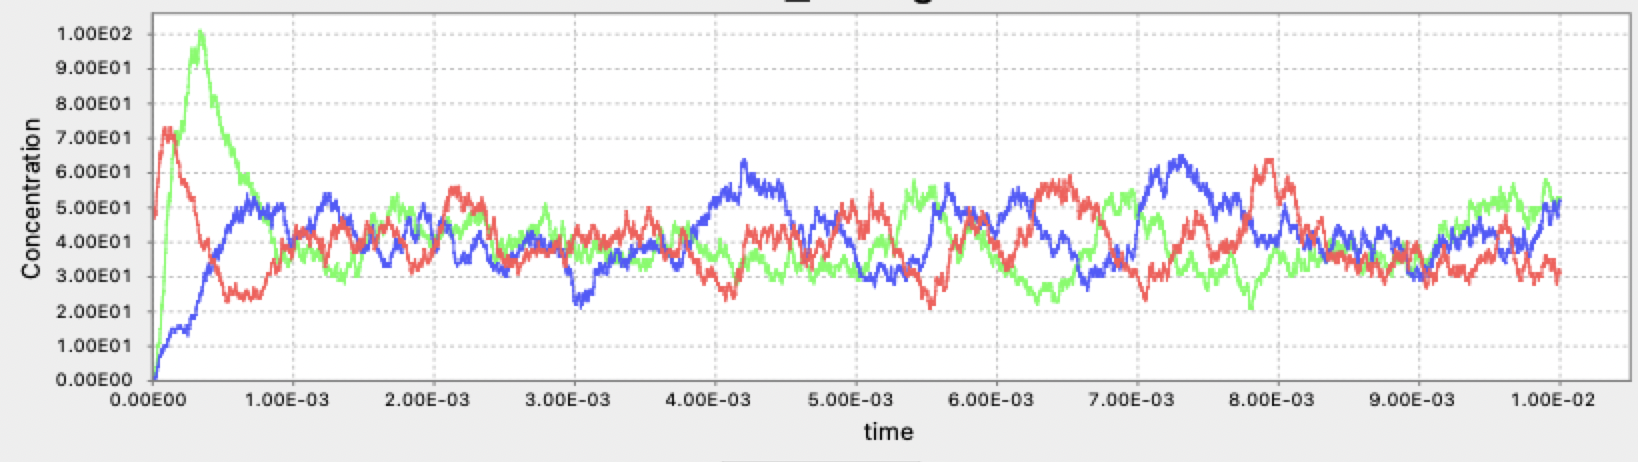
\includegraphics[width = 0.85\textwidth]{../images/nf_sim_interrupted_chart_spike.png}
\caption{A larger increase in the concentration of \textvar{Y} particles than in \autoref{fig:nf_sim_interrupted_chart} does not produce a substantive change in the system.}
\label{fig:nf_sim_interrupted_chart_spike}
\end{figure}

The repressilator is not the only network motif that leads to oscillations of particle concentrations, but robustness to disturbance is a shared feature of all these motifs. Furthermore, the repressilator is not the most robust oscillator that we can build. Real oscillators tend to have more than three components, and part of the reason why may be that researchers have shown that at least five reactions are typically needed to build a very robust oscillator.

The repressilator's robustness implies a bigger picture moral of biological modeling. If an underlying biological system demonstrates robustness to change, then any model of that system should also be able to withstand this change. Conversely, in biology and in life, we should be skeptical of any non-robust model of a robust system.

\FloatBarrier
\phantomsection
\subsection{Toward more complicated models of biochemical processes}

We have seen that even very simple network motifs can have a powerful effect on a cell's ability to implement elegant behavior. In the next section, we will encounter a much more involved biochemical process, with far more molecules and reactions, that is used by bacteria to cleverly (and robustly) explore their environment. In fact, we will have so many particles and so many reactions that we will need to completely rethink how we formulate our model.

\FloatBarrier
\section{Exercises}
\label{sec:exercises}
\phantomsection

\begin{exercise}[%
Test of exercise environment.
]\end{exercise}
